\setcounter{section}{3}
\section{Orthonormalbasis}

\subsection{Orthogonalprojektion}

Um die Orthonormalbasis besser zu verstehen, schauen wir uns nochmals die Orthogonalprojektion an. Grundlegend gibt uns die Orthogonalprojektion den Anteil eines Vektors der in dieselbe Richtung eines anderen Vektors zeigt. Oder bildlich:

\begin{figure*}[h!]
    \centering
    \tikzset{every picture/.style={line width=0.75pt}} %set default line width to 0.75pt        
    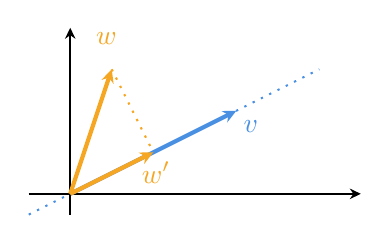
\begin{tikzpicture}[x=0.75pt,y=0.75pt,yscale=-1,xscale=1]
        %uncomment if require: \path (0,300); %set diagram left start at 0, and has height of 300

        %Straight Lines [id:da9130498050699057] 
        \draw    (260,160) -- (417,160) ;
        \draw [shift={(420,160)}, rotate = 180] [fill={rgb, 255:red, 0; green, 0; blue, 0 }  ][line width=0.08]  [draw opacity=0] (5.36,-2.57) -- (0,0) -- (5.36,2.57) -- (3.56,0) -- cycle    ;
        %Straight Lines [id:da3548240373522803] 
        \draw    (280,170) -- (280,83) ;
        \draw [shift={(280,80)}, rotate = 90] [fill={rgb, 255:red, 0; green, 0; blue, 0 }  ][line width=0.08]  [draw opacity=0] (5.36,-2.57) -- (0,0) -- (5.36,2.57) -- (3.56,0) -- cycle    ;
        %Straight Lines [id:da48897763778145353] 
        \draw [color={rgb, 255:red, 74; green, 144; blue, 226 }  ,draw opacity=1 ] [dash pattern={on 0.84pt off 2.51pt}]  (260,170) -- (400,100) ;
        %Straight Lines [id:da18358818449452052] 
        \draw [color={rgb, 255:red, 74; green, 144; blue, 226 }  ,draw opacity=1 ][line width=1.5]    (280,160) -- (356.42,121.79) ;
        \draw [shift={(360,120)}, rotate = 153.43] [fill={rgb, 255:red, 74; green, 144; blue, 226 }  ,fill opacity=1 ][line width=0.08]  [draw opacity=0] (6.43,-3.09) -- (0,0) -- (6.43,3.09) -- (4.27,0) -- cycle    ;
        %Straight Lines [id:da11243680679950874] 
        \draw [color={rgb, 255:red, 245; green, 166; blue, 35 }  ,draw opacity=1 ] [dash pattern={on 0.84pt off 2.51pt}]  (300,100) -- (320,140) ;
        %Straight Lines [id:da3605745978899313] 
        \draw [color={rgb, 255:red, 245; green, 166; blue, 35 }  ,draw opacity=1 ][line width=1.5]    (280,160) -- (298.74,103.79) ;
        \draw [shift={(300,100)}, rotate = 108.43] [fill={rgb, 255:red, 245; green, 166; blue, 35 }  ,fill opacity=1 ][line width=0.08]  [draw opacity=0] (6.43,-3.09) -- (0,0) -- (6.43,3.09) -- (4.27,0) -- cycle    ;
        %Straight Lines [id:da9560780419471896] 
        \draw [color={rgb, 255:red, 245; green, 166; blue, 35 }  ,draw opacity=1 ][line width=1.5]    (280,160) -- (316.42,141.79) ;
        \draw [shift={(320,140)}, rotate = 153.43] [fill={rgb, 255:red, 245; green, 166; blue, 35 }  ,fill opacity=1 ][line width=0.08]  [draw opacity=0] (6.43,-3.09) -- (0,0) -- (6.43,3.09) -- (4.27,0) -- cycle    ;

        % Text Node
        \draw (362,123) node [anchor=north west][inner sep=0.75pt]  [color={rgb, 255:red, 74; green, 144; blue, 226 }  ,opacity=1 ] [align=left] {$\displaystyle v$};
        % Text Node
        \draw (291,81) node [anchor=north west][inner sep=0.75pt]  [color={rgb, 255:red, 245; green, 166; blue, 35 }  ,opacity=1 ] [align=left] {$\displaystyle w$};
        % Text Node
        \draw (313,143) node [anchor=north west][inner sep=0.75pt]  [color={rgb, 255:red, 245; green, 166; blue, 35 }  ,opacity=1 ] [align=left] {$\displaystyle w'$};
    \end{tikzpicture}
\end{figure*}

Hier projizieren wir den Vektor \( w \) orthogonal auf den Vektor \( v \). Das Resultat ist der Vektor \( w' \). Mathematisch lässt sich das mit dem Skalarprodukt ausrechnen 

\begin{equation*}
    w' = \frac{\langle w, v \rangle}{\langle v, v \rangle} \ v. 
\end{equation*}

\subsection{Orthonormalbasis}

Wenn wir eine Basis für einen Vektorraum wählen, ist es vorteilhaft, wenn diese bestimmte Eigenschaften erfüllt. Eine dieser wünschenswerten Eigenschaften ist das die Basis orthonormal ist. Aber was bedeutet es, wenn eine Basis orthonormal ist, und warum ist das wünschenswert?

\vspace{1\baselineskip}

Bei einer Orthonormalbasis stehen die Basisvektoren senkrecht aufeinander (orthogonal) und haben die Länge 1 (normal). Zum Beispiel ist die Standardbasis

\begin{equation*}
    \mathcal{E} = \left\{
    e_1 =\begin{pmatrix}
        1 \\ 0
    \end{pmatrix},
    e_2 = \begin{pmatrix}
        0 \\ 1
    \end{pmatrix} \right\}, 
\end{equation*}

\vspace{0.25\baselineskip}

eine Orthonormalbasis. Wenn wir in einer solchen Basis die Koordinaten von einem Vektor \( v \) finden wollen, können wir einfach den Vektor orthogonal auf die Basisvektoren projizieren. Nehmen wir Beispielsweise den blauen Vektor \( v \) in der folgenden Abbildung:

\begin{figure*}[h!]
    \centering
    \tikzset{every picture/.style={line width=0.75pt}} %set default line width to 0.75pt        
    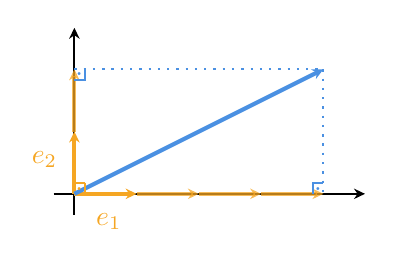
\begin{tikzpicture}[x=0.75pt,y=0.75pt,yscale=-1,xscale=1]
        %uncomment if require: \path (0,300); %set diagram left start at 0, and has height of 300

        %Straight Lines [id:da44328726608934177] 
        \draw    (250,140) -- (397,140) ;
        \draw [shift={(400,140)}, rotate = 180] [fill={rgb, 255:red, 0; green, 0; blue, 0 }  ][line width=0.08]  [draw opacity=0] (5.36,-2.57) -- (0,0) -- (5.36,2.57) -- (3.56,0) -- cycle    ;
        %Straight Lines [id:da47312587398756434] 
        \draw    (260,150) -- (260,63) ;
        \draw [shift={(260,60)}, rotate = 90] [fill={rgb, 255:red, 0; green, 0; blue, 0 }  ][line width=0.08]  [draw opacity=0] (5.36,-2.57) -- (0,0) -- (5.36,2.57) -- (3.56,0) -- cycle    ;
        %Straight Lines [id:da8659898516941857] 
        \draw [color={rgb, 255:red, 245; green, 166; blue, 35 }  ,draw opacity=1 ][line width=1.5]   (260,140) -- (287,140) ;
        \draw [shift={(290,140)}, rotate = 180] [fill={rgb, 255:red, 245; green, 166; blue, 35 }  ,fill opacity=1 ][line width=0.08]  [draw opacity=0] (5.36,-2.57) -- (0,0) -- (5.36,2.57) -- (3.56,0) -- cycle    ;
        %Straight Lines [id:da9568225102519602] 
        \draw [color={rgb, 255:red, 245; green, 166; blue, 35 }  ,draw opacity=0.75 ]  [line width=1.5] (290,140) -- (317,140) ;
        \draw [shift={(320,140)}, rotate = 180] [fill={rgb, 255:red, 245; green, 166; blue, 35 }  ,fill opacity=0.75 ][line width=0.08]  [draw opacity=0] (5.36,-2.57) -- (0,0) -- (5.36,2.57) -- (3.56,0) -- cycle    ;
        %Straight Lines [id:da5897956759571951] 
        \draw [color={rgb, 255:red, 245; green, 166; blue, 35 }  ,draw opacity=0.75 ] [line width=1.5]  (320,140) -- (347,140) ;
        \draw [shift={(350,140)}, rotate = 180] [fill={rgb, 255:red, 245; green, 166; blue, 35 }  ,fill opacity=0.75 ][line width=0.08]  [draw opacity=0] (5.36,-2.57) -- (0,0) -- (5.36,2.57) -- (3.56,0) -- cycle    ;
        %Straight Lines [id:da10531462420857163] 
        \draw [color={rgb, 255:red, 245; green, 166; blue, 35 }  ,draw opacity=0.75 ] [line width=1.5]  (350,140) -- (377,140) ;
        \draw [shift={(380,140)}, rotate = 180] [fill={rgb, 255:red, 245; green, 166; blue, 35 }  ,fill opacity=0.75 ][line width=0.08]  [draw opacity=0] (5.36,-2.57) -- (0,0) -- (5.36,2.57) -- (3.56,0) -- cycle    ;
        %Straight Lines [id:da1844149306032643] 
        \draw [color={rgb, 255:red, 245; green, 166; blue, 35 }  ,draw opacity=1 ] [line width=1.5]   (260,140) -- (260,113) ;
        \draw [shift={(260,110)}, rotate = 90] [fill={rgb, 255:red, 245; green, 166; blue, 35 }  ,fill opacity=1 ][line width=0.08]  [draw opacity=0] (5.36,-2.57) -- (0,0) -- (5.36,2.57) -- (3.56,0) -- cycle    ;
        %Straight Lines [id:da8638725124260854] 
        \draw [color={rgb, 255:red, 245; green, 166; blue, 35 }  ,draw opacity=0.75 ]  [line width=1.5] (260,110) -- (260,83) ;
        \draw [shift={(260,80)}, rotate = 90] [fill={rgb, 255:red, 245; green, 166; blue, 35 }  ,fill opacity=0.75 ][line width=0.08]  [draw opacity=0] (5.36,-2.57) -- (0,0) -- (5.36,2.57) -- (3.56,0) -- cycle    ;
        %Straight Lines [id:da8915754240181588] 
        \draw [color={rgb, 255:red, 74; green, 144; blue, 226 }  ,draw opacity=1 ] [dash pattern={on 0.84pt off 2.51pt}]  (260,80) -- (380,80) ;
        %Straight Lines [id:da5199302106092814] 
        \draw [color={rgb, 255:red, 74; green, 144; blue, 226 }  ,draw opacity=1 ] [dash pattern={on 0.84pt off 2.51pt}]  (380,80) -- (380,140) ;
        %Straight Lines [id:da7243997817117014] 
        \draw [color={rgb, 255:red, 74; green, 144; blue, 226 }  ,draw opacity=1 ] [line width=1.5]   (260,140) -- (377.32,81.34) ;
        \draw [shift={(380,80)}, rotate = 153.43] [fill={rgb, 255:red, 74; green, 144; blue, 226 }  ,fill opacity=1 ][line width=0.08]  [draw opacity=0] (5.36,-2.57) -- (0,0) -- (5.36,2.57) -- (3.56,0) -- cycle    ;
        %Straight Lines [id:da514228479352661] 
        \draw [color={rgb, 255:red, 74; green, 144; blue, 226 }  ,draw opacity=1 ]   (260,85) -- (265,85) ;
        %Straight Lines [id:da8876355618505145] 
        \draw [color={rgb, 255:red, 74; green, 144; blue, 226 }  ,draw opacity=1 ]   (374.6,135) -- (380,135) ;
        %Straight Lines [id:da4612659871711752] 
        \draw [color={rgb, 255:red, 74; green, 144; blue, 226 }  ,draw opacity=1 ]   (375,135) -- (375,140) ;
        %Straight Lines [id:da3865777958473725] 
        \draw [color={rgb, 255:red, 74; green, 144; blue, 226 }  ,draw opacity=1 ]   (265,80) -- (265,85.4) ;
        %Straight Lines [id:da10089672630697488] 
        \draw [color={rgb, 255:red, 245; green, 166; blue, 35 }  ,draw opacity=1 ]   (265,134.6) -- (265,140) ;
        %Straight Lines [id:da186138120295385] 
        \draw [color={rgb, 255:red, 245; green, 166; blue, 35 }  ,draw opacity=1 ]   (260,135) -- (265,135) ;

        % Text Node
        \draw (269,148) node [anchor=north west][inner sep=0.75pt]  [color={rgb, 255:red, 245; green, 166; blue, 35 }  ,opacity=1 ] [align=left] {$\displaystyle e_{1}$};
        % Text Node
        \draw (238,118) node [anchor=north west][inner sep=0.75pt]  [color={rgb, 255:red, 245; green, 166; blue, 35 }  ,opacity=1 ] [align=left] {$\displaystyle e_{2}$};
        % Text Node
        \draw (259,135.5) node [anchor=north west][inner sep=0.75pt]  [color={rgb, 255:red, 245; green, 166; blue, 35 }  ,opacity=1 ] [align=left] {.};
        % Text Node
        \draw (374,135.5) node [anchor=north west][inner sep=0.75pt]  [color={rgb, 255:red, 74; green, 144; blue, 226 }  ,opacity=1 ] [align=left] {.};
        % Text Node
        \draw (259,80) node [anchor=north west][inner sep=0.75pt]  [color={rgb, 255:red, 74; green, 144; blue, 226 }  ,opacity=1 ] [align=left] {.};
    \end{tikzpicture}
\end{figure*}

Durch die Orthogonalprojektionen auf die Basisvektoren erhalten wir die Koordinaten von \( v \) in der Basis \( \mathcal{E} \). In diesem Fall sind die Koordinaten gegeben durch

\begin{equation*}
    v = \left[ \begin{pmatrix} 4 \\ 2 \end{pmatrix} \right]_\mathcal{E}. 
\end{equation*}

\vspace{0.25\baselineskip}

Bei einer nicht orthonormalen Basis müssen die Basisvektoren weder orthogonal noch normiert sein. Zum Beispiel

\begin{equation*}
    \mathcal{B} = \left\{
    b_1 =\begin{pmatrix}
        1 \\ - \frac{1}{2}
    \end{pmatrix}
    \text{ und }
    b_2 = \begin{pmatrix}
        1 \\ 1
    \end{pmatrix} \right\}. 
\end{equation*}

\vspace{0.25\baselineskip}

Versuchen wir nun die Koordinaten desselben Vektors \( v \) in dieser Basis \( \mathcal{B} \) zu finden. Wieder projizieren wir den Vektor \( v \) orthogonal auf die Basisvektoren. 

\begin{figure*}[h!]
    \centering
    \tikzset{every picture/.style={line width=0.75pt}} %set default line width to 0.75pt        
    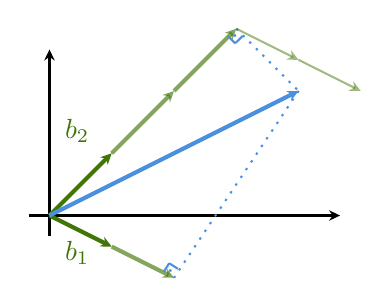
\begin{tikzpicture}[x=0.75pt,y=0.75pt,yscale=-1,xscale=1]
        %uncomment if require: \path (0,300); %set diagram left start at 0, and has height of 300
        %Straight Lines [id:da44328726608934177] 
        \draw    (250,140) -- (397,140) ;
        \draw [shift={(400,140)}, rotate = 180] [fill={rgb, 255:red, 0; green, 0; blue, 0 }  ][line width=0.08]  [draw opacity=0] (5.36,-2.57) -- (0,0) -- (5.36,2.57) -- (3.56,0) -- cycle    ;
        %Straight Lines [id:da47312587398756434] 
        \draw    (260,150) -- (260,63) ;
        \draw [shift={(260,60)}, rotate = 90] [fill={rgb, 255:red, 0; green, 0; blue, 0 }  ][line width=0.08]  [draw opacity=0] (5.36,-2.57) -- (0,0) -- (5.36,2.57) -- (3.56,0) -- cycle    ;
        %Straight Lines [id:da8659898516941857] 
        \draw [color={rgb, 255:red, 65; green, 117; blue, 5 }  ,draw opacity=1 ]  [line width=1.5] (260,140) -- (287.32,153.66) ;
        \draw [shift={(290,155)}, rotate = 206.57] [fill={rgb, 255:red, 65; green, 117; blue, 5 }  ,fill opacity=1 ][line width=0.08]  [draw opacity=0] (5.36,-2.57) -- (0,0) -- (5.36,2.57) -- (3.56,0) -- cycle    ;
        %Straight Lines [id:da1844149306032643] 
        \draw [color={rgb, 255:red, 65; green, 117; blue, 5 }  ,draw opacity=1 ] [line width=1.5]  (260,140) -- (287.88,112.12) ;
        \draw [shift={(290,110)}, rotate = 135] [fill={rgb, 255:red, 65; green, 117; blue, 5 }  ,fill opacity=1 ][line width=0.08]  [draw opacity=0] (5.36,-2.57) -- (0,0) -- (5.36,2.57) -- (3.56,0) -- cycle    ;
        %Straight Lines [id:da8915754240181588] 
        \draw [color={rgb, 255:red, 74; green, 144; blue, 226 }  ,draw opacity=1 ] [dash pattern={on 0.84pt off 2.51pt}]  (350,50) -- (380,80) ;
        %Straight Lines [id:da5199302106092814] 
        \draw [color={rgb, 255:red, 74; green, 144; blue, 226 }  ,draw opacity=1 ] [dash pattern={on 0.84pt off 2.51pt}]  (380,80) -- (320,170) ;
        %Straight Lines [id:da7243997817117014] 
        \draw [color={rgb, 255:red, 74; green, 144; blue, 226 }  ,draw opacity=1 ] [line width=1.5]  (260,140) -- (377.32,81.34) ;
        \draw [shift={(380,80)}, rotate = 153.43] [fill={rgb, 255:red, 74; green, 144; blue, 226 }  ,fill opacity=1 ][line width=0.08]  [draw opacity=0] (5.36,-2.57) -- (0,0) -- (5.36,2.57) -- (3.56,0) -- cycle    ;
        %Straight Lines [id:da7517987574157674] 
        \draw [color={rgb, 255:red, 65; green, 117; blue, 5 }  ,draw opacity=0.65 ] [line width=1.5]  (290,155) -- (317.32,168.66) ;
        \draw [shift={(320,170)}, rotate = 206.57] [fill={rgb, 255:red, 65; green, 117; blue, 5 }  ,fill opacity=0.65 ][line width=0.08]  [draw opacity=0] (5.36,-2.57) -- (0,0) -- (5.36,2.57) -- (3.56,0) -- cycle    ;
        %Straight Lines [id:da07863847158468451] 
        \draw [color={rgb, 255:red, 65; green, 117; blue, 5 }  ,draw opacity=0.65 ] [line width=1.5]  (290,110) -- (317.88,82.12) ;
        \draw [shift={(320,80)}, rotate = 135] [fill={rgb, 255:red, 65; green, 117; blue, 5 }  ,fill opacity=0.65 ][line width=0.08]  [draw opacity=0] (5.36,-2.57) -- (0,0) -- (5.36,2.57) -- (3.56,0) -- cycle    ;
        %Straight Lines [id:da616873264881425] 
        \draw [color={rgb, 255:red, 65; green, 117; blue, 5 }  ,draw opacity=0.65 ]  [line width=1.5] (320,80) -- (347.88,52.12) ;
        \draw [shift={(350,50)}, rotate = 135] [fill={rgb, 255:red, 65; green, 117; blue, 5 }  ,fill opacity=0.65 ][line width=0.08]  [draw opacity=0] (5.36,-2.57) -- (0,0) -- (5.36,2.57) -- (3.56,0) -- cycle    ;
        %Straight Lines [id:da7636253123951711] 
        \draw [color={rgb, 255:red, 74; green, 144; blue, 226 }  ,draw opacity=1 ]   (349.46,57.04) -- (353.04,53.54) ;
        %Straight Lines [id:da6601484607060893] 
        \draw [color={rgb, 255:red, 74; green, 144; blue, 226 }  ,draw opacity=1 ]   (349.46,57.04) -- (345.96,53.46) ;
        %Straight Lines [id:da14727540501130232] 
        \draw [color={rgb, 255:red, 74; green, 144; blue, 226 }  ,draw opacity=1 ]   (317.68,163) -- (321.9,165.68) ;
        %Straight Lines [id:da7371410939351042] 
        \draw [color={rgb, 255:red, 74; green, 144; blue, 226 }  ,draw opacity=1 ]   (317.68,163) -- (315,167.22) ;
        %Straight Lines [id:da219327386047809] 
        \draw [color={rgb, 255:red, 65; green, 117; blue, 5 }  ,draw opacity=0.5 ]   (350,50) -- (377.32,63.66) ;
        \draw [shift={(380,65)}, rotate = 206.57] [fill={rgb, 255:red, 65; green, 117; blue, 5 }  ,fill opacity=0.5 ][line width=0.08]  [draw opacity=0] (5.36,-2.57) -- (0,0) -- (5.36,2.57) -- (3.56,0) -- cycle    ;
        %Straight Lines [id:da3698728532056801] 
        \draw [color={rgb, 255:red, 65; green, 117; blue, 5 }  ,draw opacity=0.5 ]   (380,65) -- (407.32,78.66) ;
        \draw [shift={(410,80)}, rotate = 206.57] [fill={rgb, 255:red, 65; green, 117; blue, 5 }  ,fill opacity=0.5 ][line width=0.08]  [draw opacity=0] (5.36,-2.57) -- (0,0) -- (5.36,2.57) -- (3.56,0) -- cycle    ;
        
        % Text Node
        \draw (266,92) node [anchor=north west][inner sep=0.75pt]  [color={rgb, 255:red, 245; green, 166; blue, 35 }  ,opacity=1 ] [align=left] {$\displaystyle \textcolor[rgb]{0.25,0.46,0.02}{b_{2}}$};
        % Text Node
        \draw (266,151) node [anchor=north west][inner sep=0.75pt]  [color={rgb, 255:red, 245; green, 166; blue, 35 }  ,opacity=1 ] [align=left] {$\displaystyle \textcolor[rgb]{0.25,0.46,0.02}{b}\textcolor[rgb]{0.25,0.46,0.02}{_{1}}$};
        % Text Node
        \draw (346,51.5) node [anchor=north west][inner sep=0.75pt]  [color={rgb, 255:red, 74; green, 144; blue, 226 }  ,opacity=1 ] [align=left] {.};
        % Text Node
        \draw (315,164.5) node [anchor=north west][inner sep=0.75pt]  [color={rgb, 255:red, 74; green, 144; blue, 226 }  ,opacity=1 ] [align=left] {.};
    \end{tikzpicture}
\end{figure*}

Durch die Orthogonalprojektion erhalten wir die Koordinaten \( \begin{bmatrix} 2 & 3 \end{bmatrix}^\intercal \). Diese entsprechen jedoch nicht dem Vektor \( v \). 

\begin{equation*}
    v \neq \left[ \begin{pmatrix} 2 \\ 3 \end{pmatrix} \right]_\mathcal{B}.
\end{equation*}

\vspace{0.25\baselineskip}

Wenn wir einen Vektor in einer solchen nicht-orthogonalen Basis darstellen wollen, dann können wir nicht einfach orthogonal projizieren. Um die entsprechenden Koordinaten zu finden, müssen wir eine Linearkombination der Basisvektoren finden (LGS lösen). 

\vspace{1\baselineskip}

Für unsere Orthonormalbasis bedeutet das nun folgendes. Sei \( \mathcal{E} = \{ e_1, e_2, \ldots, e_n \} \) eine Orthonormalbasis des Vektorraums \( V \), dann gilt \( \forall x \in V \)

\begin{equation*}
    x = \sum_{k=1}^n \langle x, e_k \rangle e_k.
\end{equation*}

\vspace{0.25\baselineskip}

In anderen Worten, können wir jeden Vektor als Linearkombination der Basisvektoren schreiben, wobei die Koeffizienten durch die Orthogonalprojektionen gegeben sind. Um die Koordinaten zu finden, müssen wir kein LGS lösen. Beachte das der Term \( \langle e_k, e_k \rangle \) wegfällt, da dieser aufgrund der Normierung immer 1 ist.

\subsection{Gram-Schmidt-Orthogonalisierungsverfahren}

Aufgrund der oben genannten Eigenschaften wollen wir oft mit Orthonormalbasen arbeiten. Um eine solche Basis zu finden, benutzten wir das Gram Schmidt Orthogonalisierungsverfahren. Dieses Verfahren erlaubt uns aus einer jeder Basis eine Orthonormalbasis zu erstellen. Dafür benötigen wir eine beliebige Basis \( \mathcal{B} = \{ b_1, \ldots, b_k \} \) und ein Skalarprodukt, mit welchen wir dann eine Orthonormalbasis \( \mathcal{E} = \{ e_1, \ldots, e_k \} \) erstellen. Im Folgenden gehen wir das Verfahren Schritt für Schritt durch.

\newpage

\begin{enumerate}
    \item Wähle einen beliebigen Basisvektor \( b_1 \) und normiere ihn. 
    
    \begin{figure*}[h!]
        \begin{minipage}{0.49\textwidth}    
            \begin{equation*}
                e_1 = \frac{b_1}{\| b_1 \|} = \frac{b_1}{\sqrt{\langle b_1, b_1 \rangle}}
            \end{equation*}
        \end{minipage}
        \begin{minipage}{0.5\textwidth}
            \centering
            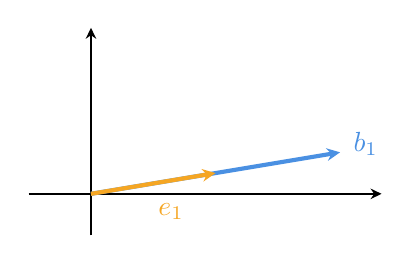
\begin{tikzpicture}[x=0.75pt,y=0.75pt,yscale=-1,xscale=1]
                %uncomment if require: \path (0,300); %set diagram left start at 0, and has height of 300
                %Straight Lines [id:da9130498050699057] 
                \draw    (250,160) -- (417,160) ;
                \draw [shift={(420,160)}, rotate = 180] [fill={rgb, 255:red, 0; green, 0; blue, 0 }  ][line width=0.08]  [draw opacity=0] (5.36,-2.57) -- (0,0) -- (5.36,2.57) -- (3.56,0) -- cycle    ;
                %Straight Lines [id:da3548240373522803] 
                \draw    (280,180) -- (280,83) ;
                \draw [shift={(280,80)}, rotate = 90] [fill={rgb, 255:red, 0; green, 0; blue, 0 }  ][line width=0.08]  [draw opacity=0] (5.36,-2.57) -- (0,0) -- (5.36,2.57) -- (3.56,0) -- cycle    ;
                %Straight Lines [id:da18358818449452052] 
                \draw [color={rgb, 255:red, 74; green, 144; blue, 226 }  ,draw opacity=1 ][line width=1.5]    (280,160) -- (396.05,140.66) ;
                \draw [shift={(400,140)}, rotate = 170.54] [fill={rgb, 255:red, 74; green, 144; blue, 226 }  ,fill opacity=1 ][line width=0.08]  [draw opacity=0] (6.43,-3.09) -- (0,0) -- (6.43,3.09) -- (4.27,0) -- cycle    ;
                %Straight Lines [id:da9560780419471896] 
                \draw [color={rgb, 255:red, 245; green, 166; blue, 35 }  ,draw opacity=1 ][line width=1.5]    (280,160) -- (336.05,150.66) ;
                \draw [shift={(340,150)}, rotate = 170.54] [fill={rgb, 255:red, 245; green, 166; blue, 35 }  ,fill opacity=1 ][line width=0.08]  [draw opacity=0] (6.43,-3.09) -- (0,0) -- (6.43,3.09) -- (4.27,0) -- cycle    ;
        
                % Text Node
                \draw (405,129) node [anchor=north west][inner sep=0.75pt]  [color={rgb, 255:red, 74; green, 144; blue, 226 }  ,opacity=1 ] [align=left] {$\displaystyle b_{1}$};
                % Text Node
                \draw (311,163) node [anchor=north west][inner sep=0.75pt]  [color={rgb, 255:red, 245; green, 166; blue, 35 }  ,opacity=1 ] [align=left] {$\displaystyle e_{1}$};
            \end{tikzpicture}
        \end{minipage}
    \end{figure*}
    

    \item Wähle einen zweiten Basisvektor \( b_2 \), ziehe zuerst den zu \( e_1 \)  parallelen Teil ab
    
    \begin{figure*}[h!]
        \begin{minipage}{0.49\textwidth}
            \begin{equation*}
                e_2' = b_2 - \underbrace{\langle b_2, e_1 \rangle e_1}_{v}
            \end{equation*}
        \end{minipage}
        \begin{minipage}{0.5\textwidth}
            \centering
            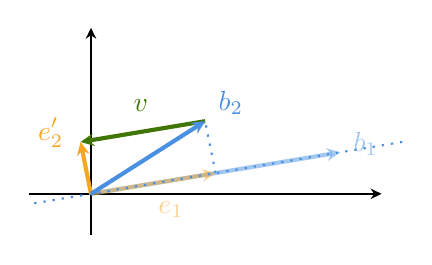
\begin{tikzpicture}[x=0.75pt,y=0.75pt,yscale=-1,xscale=1]
                %uncomment if require: \path (0,300); %set diagram left start at 0, and has height of 300
                %Straight Lines [id:da9130498050699057] 
                \draw    (250,160) -- (417,160) ;
                \draw [shift={(420,160)}, rotate = 180] [fill={rgb, 255:red, 0; green, 0; blue, 0 }  ][line width=0.08]  [draw opacity=0] (5.36,-2.57) -- (0,0) -- (5.36,2.57) -- (3.56,0) -- cycle    ;
                %Straight Lines [id:da3548240373522803] 
                \draw    (280,180) -- (280,83) ;
                \draw [shift={(280,80)}, rotate = 90] [fill={rgb, 255:red, 0; green, 0; blue, 0 }  ][line width=0.08]  [draw opacity=0] (5.36,-2.57) -- (0,0) -- (5.36,2.57) -- (3.56,0) -- cycle    ;
                %Straight Lines [id:da18358818449452052] 
                \draw [color={rgb, 255:red, 74; green, 144; blue, 226 }  ,draw opacity=0.5 ][line width=1.5]    (280,160) -- (396.05,140.66) ;
                \draw [shift={(400,140)}, rotate = 170.54] [fill={rgb, 255:red, 74; green, 144; blue, 226 }  ,fill opacity=0.5 ][line width=0.08]  [draw opacity=0] (6.43,-3.09) -- (0,0) -- (6.43,3.09) -- (4.27,0) -- cycle    ;
                %Straight Lines [id:da9560780419471896] 
                \draw [color={rgb, 255:red, 245; green, 166; blue, 35 }  ,draw opacity=0.5 ][line width=1.5]    (280,160) -- (336.05,150.66) ;
                \draw [shift={(340,150)}, rotate = 170.54] [fill={rgb, 255:red, 245; green, 166; blue, 35 }  ,fill opacity=0.5 ][line width=0.08]  [draw opacity=0] (6.43,-3.09) -- (0,0) -- (6.43,3.09) -- (4.27,0) -- cycle    ;
                %Straight Lines [id:da5390513876892769] 
                \draw [color={rgb, 255:red, 74; green, 144; blue, 226 }  ,draw opacity=1 ] [dash pattern={on 0.84pt off 2.51pt}]  (430,135) -- (250,165) ;
                %Straight Lines [id:da11486103917361612] 
                \draw [color={rgb, 255:red, 74; green, 144; blue, 226 }  ,draw opacity=1 ] [dash pattern={on 0.84pt off 2.51pt}]  (340,150) -- (335,125) ;
                %Straight Lines [id:da32074261677418026] 
                \draw [color={rgb, 255:red, 65; green, 117; blue, 5 }  ,draw opacity=1 ][line width=1.5]    (278.95,134.34) -- (335,125) ;
                \draw [shift={(275,135)}, rotate = 350.54] [fill={rgb, 255:red, 65; green, 117; blue, 5 }  ,fill opacity=1 ][line width=0.08]  [draw opacity=0] (6.43,-3.09) -- (0,0) -- (6.43,3.09) -- (4.27,0) -- cycle    ;
                %Straight Lines [id:da44202118240105737] 
                \draw [color={rgb, 255:red, 245; green, 166; blue, 35 }  ,draw opacity=1 ][line width=1.5]    (280,160) -- (275.78,138.92) ;
                \draw [shift={(275,135)}, rotate = 78.69] [fill={rgb, 255:red, 245; green, 166; blue, 35 }  ,fill opacity=1 ][line width=0.08]  [draw opacity=0] (6.43,-3.09) -- (0,0) -- (6.43,3.09) -- (4.27,0) -- cycle    ;
                %Straight Lines [id:da34733901937251044] 
                \draw [color={rgb, 255:red, 74; green, 144; blue, 226 }  ,draw opacity=1 ][line width=1.5]    (280,160) -- (331.63,127.15) ;
                \draw [shift={(335,125)}, rotate = 147.53] [fill={rgb, 255:red, 74; green, 144; blue, 226 }  ,fill opacity=1 ][line width=0.08]  [draw opacity=0] (6.43,-3.09) -- (0,0) -- (6.43,3.09) -- (4.27,0) -- cycle    ;
    
                % Text Node
                \draw (405,129) node [anchor=north west][inner sep=0.75pt]  [color={rgb, 255:red, 74; green, 144; blue, 226 }  ,opacity=0.5 ] [align=left] {$\displaystyle b_{1}$};
                % Text Node
                \draw (311,162) node [anchor=north west][inner sep=0.75pt]  [color={rgb, 255:red, 245; green, 166; blue, 35 }  ,opacity=0.5 ] [align=left] {$\displaystyle e_{1}$};
                % Text Node
                \draw (340,109) node [anchor=north west][inner sep=0.75pt]  [color={rgb, 255:red, 74; green, 144; blue, 226 }  ,opacity=1 ] [align=left] {$\displaystyle b_{2}$};
                % Text Node
                \draw (253,122) node [anchor=north west][inner sep=0.75pt]  [color={rgb, 255:red, 245; green, 166; blue, 35 }  ,opacity=1 ] [align=left] {$\displaystyle e'_{2}$};
                % Text Node
                \draw (299,113) node [anchor=north west][inner sep=0.75pt]  [color={rgb, 255:red, 65; green, 117; blue, 5 }  ,opacity=1 ] [align=left] {$\displaystyle v$};
            \end{tikzpicture}
        \end{minipage}
    \end{figure*}

    und normiere ihn dann

    \begin{figure*}[h!]
        \begin{minipage}{0.49\textwidth}
            \begin{equation*}
                e_2 = \frac{e_2'}{\| e_2' \|} = \frac{e_2'}{\sqrt{\langle e_2', e_2' \rangle}}
            \end{equation*}        
        \end{minipage}
        \begin{minipage}{0.5\textwidth}
            \centering
            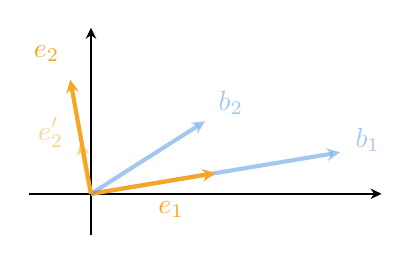
\begin{tikzpicture}[x=0.75pt,y=0.75pt,yscale=-1,xscale=1]
                %uncomment if require: \path (0,300); %set diagram left start at 0, and has height of 300
                
                %Straight Lines [id:da9130498050699057] 
                \draw    (250,160) -- (417,160) ;
                \draw [shift={(420,160)}, rotate = 180] [fill={rgb, 255:red, 0; green, 0; blue, 0 }  ][line width=0.08]  [draw opacity=0] (5.36,-2.57) -- (0,0) -- (5.36,2.57) -- (3.56,0) -- cycle    ;
                %Straight Lines [id:da3548240373522803] 
                \draw    (280,180) -- (280,83) ;
                \draw [shift={(280,80)}, rotate = 90] [fill={rgb, 255:red, 0; green, 0; blue, 0 }  ][line width=0.08]  [draw opacity=0] (5.36,-2.57) -- (0,0) -- (5.36,2.57) -- (3.56,0) -- cycle    ;
                %Straight Lines [id:da18358818449452052] 
                \draw [color={rgb, 255:red, 74; green, 144; blue, 226 }  ,draw opacity=0.5 ][line width=1.5]    (280,160) -- (396.05,140.66) ;
                \draw [shift={(400,140)}, rotate = 170.54] [fill={rgb, 255:red, 74; green, 144; blue, 226 }  ,fill opacity=0.5 ][line width=0.08]  [draw opacity=0] (6.43,-3.09) -- (0,0) -- (6.43,3.09) -- (4.27,0) -- cycle    ;
                %Straight Lines [id:da9560780419471896] 
                \draw [color={rgb, 255:red, 245; green, 166; blue, 35 }  ,draw opacity=1 ][line width=1.5]    (280,160) -- (336.05,150.66) ;
                \draw [shift={(340,150)}, rotate = 170.54] [fill={rgb, 255:red, 245; green, 166; blue, 35 }  ,fill opacity=1 ][line width=0.08]  [draw opacity=0] (6.43,-3.09) -- (0,0) -- (6.43,3.09) -- (4.27,0) -- cycle    ;
                %Straight Lines [id:da34733901937251044] 
                \draw [color={rgb, 255:red, 74; green, 144; blue, 226 }  ,draw opacity=0.5 ][line width=1.5]    (280,160) -- (331.63,127.15) ;
                \draw [shift={(335,125)}, rotate = 147.53] [fill={rgb, 255:red, 74; green, 144; blue, 226 }  ,fill opacity=0.5 ][line width=0.08]  [draw opacity=0] (6.43,-3.09) -- (0,0) -- (6.43,3.09) -- (4.27,0) -- cycle    ;
                %Straight Lines [id:da9237343905439186] 
                \draw [color={rgb, 255:red, 245; green, 166; blue, 35 }  ,draw opacity=1 ][line width=1.5]    (280,160) -- (271.19,111.56) -- (270.72,108.94) ;
                \draw [shift={(270,105)}, rotate = 79.7] [fill={rgb, 255:red, 245; green, 166; blue, 35 }  ,fill opacity=1 ][line width=0.08]  [draw opacity=0] (6.43,-3.09) -- (0,0) -- (6.43,3.09) -- (4.27,0) -- cycle    ;
                %Straight Lines [id:da9153064885684233] 
                \draw [color={rgb, 255:red, 245; green, 166; blue, 35 }  ,draw opacity=0.5 ][line width=1.5]    (280,160) -- (275.78,138.92) ;
                \draw [shift={(275,135)}, rotate = 78.69] [fill={rgb, 255:red, 245; green, 166; blue, 35 }  ,fill opacity=0.5 ][line width=0.08]  [draw opacity=0] (6.43,-3.09) -- (0,0) -- (6.43,3.09) -- (4.27,0) -- cycle    ;
                
                % Text Node
                \draw (406,127) node [anchor=north west][inner sep=0.75pt]  [color={rgb, 255:red, 74; green, 144; blue, 226 }  ,opacity=0.5 ] [align=left] {$\displaystyle b_{1}$};
                % Text Node
                \draw (311,162) node [anchor=north west][inner sep=0.75pt]  [color={rgb, 255:red, 245; green, 166; blue, 35 }  ,opacity=1 ] [align=left] {$\displaystyle e_{1}$};
                % Text Node
                \draw (340,109) node [anchor=north west][inner sep=0.75pt]  [color={rgb, 255:red, 74; green, 144; blue, 226 }  ,opacity=0.5 ] [align=left] {$\displaystyle b_{2}$};
                % Text Node
                \draw (253,122) node [anchor=north west][inner sep=0.75pt]  [color={rgb, 255:red, 245; green, 166; blue, 35 }  ,opacity=0.5 ] [align=left] {$\displaystyle e'_{2}$};
                % Text Node
                \draw (251,87) node [anchor=north west][inner sep=0.75pt]  [color={rgb, 255:red, 245; green, 166; blue, 35 }  ,opacity=1 ] [align=left] {$\displaystyle e_{2}$};
            \end{tikzpicture}
        \end{minipage}
    \end{figure*}

    \item Wiederhole für jeden Basisvektor \( b_i \) 
    
        \begin{equation*}
            \begin{aligned}
                e_i' &= b_i - \langle b_i, e_1 \rangle e_1 - \langle b_i, e_2 \rangle e_2 - \ldots - \langle b_i, e_{i-1} \rangle e_{i-1} \\[1em]
                e_i &= \frac{e_i'}{\| e_i' \|} = \frac{e_i'}{\sqrt{\langle e_i', e_i' \rangle}}
            \end{aligned}
        \end{equation*}
\end{enumerate}

\subsubsection*{Beispiel}

Sei auf \( \mathcal{P}_4 \) das folgende Skalarprodukt gegeben:

\begin{equation*}
    \langle p, q \rangle = \int_{0}^{1} p(x)q(x) \, dx,
\end{equation*}

\vspace{0.25\baselineskip}

finde eine Orthonormalbasis für den Vektorraum \( span \{ 1, 3x^4 \} \).

\vspace{1\baselineskip}

Wir benutzten das Gram-Schmidt-Verfahren mit den Basisvektoren \( b_1 = 1 \) und \( b_2 = 3x^4 \).

\begin{enumerate}
    \item 
    \begin{equation*}
        \begin{aligned}
            e_1 &= \frac{b_1}{\| b_1 \|} = \frac{b_1}{\sqrt{\langle b_1, b_1 \rangle}} \\[1em]
            & \qquad \to \langle b_1, b_1 \rangle = \int_{0}^{1} 1 \cdot 1 \, dx = \left[ x \right]_0^1 = 1 \\[1em]
            e_1 &= 1
        \end{aligned}
    \end{equation*}
    \item 
    \begin{equation*}
        \begin{aligned}
            e_2' &= b_2 - \langle b_2, e_1 \rangle e_1 \\[1em]
            & \qquad \to \langle b_2, e_1 \rangle = \int_{0}^{1} 3x^4 \cdot 1 \, dx = \left[ \frac{3}{5} x^5 \right]_0^1 = \frac{3}{5} \\[1em]
            e_2' &= b_2 - \frac{3}{5} = 3x^4 - \frac{3}{5} \\[2em]
            e_2 &= \frac{e_2'}{\| e_2' \|} = \frac{e_2'}{\sqrt{\langle e_2', e_2' \rangle}} \\[1em]
            & \qquad \to \langle e_2', e_2' \rangle = \int_{0}^{1} \left( 3x^4 - \frac{3}{5} \right)^2 \, dx = \int_{0}^{1} 9x^8 - \frac{18}{5}x^4 + \frac{9}{25} \, dx \\[1em]
            & \qquad \qquad \qquad \ \ = \left[ x^9 - \frac{18}{25} x^5 + \frac{9}{25} x \right]_0^1 = \frac{16}{25} \\[1em]
            & \qquad \to \sqrt{\langle e_2', e_2' \rangle} = \frac{4}{5} \\[1em]
            e_2 &= \frac{5}{4} \left(3x^4 - \frac{3}{5} \right) = \frac{15}{4}x^4 - \frac{3}{4}
        \end{aligned}
    \end{equation*}
\end{enumerate}

\vspace{1\baselineskip}

Die Orthonormalbasis ist gegeben durch 

\begin{equation*}
    \mathcal{E} = \left\{ 1, \frac{15}{4}x^4 - \frac{3}{4} \right\}.
\end{equation*}

Zusammengefasst kann das Gram-Schmidt-Verfahren in einem Kochrezept zusammengefasst werden.

\begin{tcolorbox}[colback=gray!30, colframe=gray!80, title=Gram-Schmidt-Verfahren]
    Für das Gram-Schmidt-Verfahren benötigt man eine beliebige Basis \( \mathcal{B} = \{ b_1, \ldots, b_k \} \), sowie ein beliebeiges Skalarprodukt. Daraus lässt sich dann eine Orthonormalbasis \( \mathcal{E} = \{ e_1, \ldots, e_k \} \) erstellen.
    \begin{enumerate}
        \item Wähle einen beliebeigen Basisvektor \( b_1 \) und normiere ihn mit der vom Skalarprodukt induzierten Norm.
        \begin{equation*}
            e_1 = \frac{b_1}{\| b_1 \|} = \frac{b_1}{\sqrt{\langle b_1, b_1 \rangle}}
        \end{equation*}
        \item Wähle einen zwieten Basisvektor \( b_2 \), ziehe den zu \( b_1 \) parallelen Teil ab un normiere ihn.
        \begin{equation*}
            \begin{aligned}
                e_2' &= b_2 - \langle b_2, e_1 \rangle e_1 \\[1em]
                e_2 &= \frac{e_2'}{\| e_2' \|} = \frac{e_2'}{\sqrt{\langle e_2', e_2' \rangle}}
            \end{aligned}
        \end{equation*}
        \item Wiederhole für jeden Basisvektor \( b_i \)
        \begin{equation*}
            \begin{aligned}
                e_i' &= b_i - \langle b_i, e_1 \rangle e_1 - \langle b_i, e_2 \rangle e_2 - \ldots - \langle b_i, e_{i-1} \rangle e_{i-1} \\[1em]
                e_i &= \frac{e_i'}{\| e_i' \|} = \frac{e_i'}{\sqrt{\langle e_i', e_i' \rangle}}
            \end{aligned}
        \end{equation*}
    \end{enumerate}
\end{tcolorbox}